% -*- coding: utf-8 -*-
% !TEX program = xelatex

\documentclass[9pt]{beamer}

\usetheme[style=beta]{epyt} % alpha, beta, delta, gamma, zeta
% \usetheme{Warsaw}
\usepackage[UTF8,noindent]{ctex}
\def\blue{\textcolor{blue}}
\def\red{\textcolor{red}}
\def\purple{\textcolor{purple}}
\def\ds{\displaystyle}
\def\cd{\cdots}
\def\dd{\ddots}
\def\vd{\vdots}
\def\id{\iddots}
\def\ft{\frametitle}
\def\diag{\mathrm{diag}}

\def\A{\boldsymbol{A}}
\def\B{\boldsymbol{B}}
\def\C{\boldsymbol{C}}
\def\D{\boldsymbol{D}}
\def\E{\boldsymbol{E}}
\def\F{\boldsymbol{F}}
\def\T{\boldsymbol{T}}
\def\U{\boldsymbol{U}}
\def\X{\boldsymbol{X}}
\def\Y{\boldsymbol{Y}}
\def\Z{\boldsymbol{Z}}
\def\QQ{\boldsymbol{Q}}

\def\R{\mathbb R}
\def\rank{\mathrm{R}}
\def\det{\mathrm{det}}
\def\nn{{\boldsymbol{n}}}
\def\xx{{\boldsymbol{x}}}
\def\yy{{\boldsymbol{y}}}
\def\aa{{\boldsymbol{a}}}
\def\bb{{\boldsymbol{b}}}
\def\ee{{\boldsymbol{e}}}
\def\ii{{\boldsymbol{i}}}
\def\jj{{\boldsymbol{j}}}
\def\kk{{\boldsymbol{k}}}
\def\uu{{\boldsymbol{u}}}
\def\vv{{\boldsymbol{v}}}

\def\tf{\ttfamily}
\def\zero{\boldsymbol{0}}
\def\II{\boldsymbol{I}}
\def\PP{\boldsymbol{P}}
\def\XX{\boldsymbol{X}}
\def\Lambdabd{\boldsymbol{\Lambda}}
\def\alphabd{\boldsymbol{\alpha}}
\def\betabd{\boldsymbol{\beta}}
\def\gammabd{\boldsymbol{\gamma}}
\def\xibd{\boldsymbol{\xi}}
\def\etabd{\boldsymbol{\eta}}
\def\epsilonbd{\boldsymbol{\epsilon}}
\usepackage{multicol}
%\usepackage{fontspec}
\usepackage[most]{tcolorbox}
\newcounter{testexample}
\usepackage{xparse}
\usepackage{lipsum}
\usepackage[UTF8,noindent]{ctex}
\usepackage{extarrows}
%\usepackage{courier}
\usepackage{animate}
\usepackage{dcolumn}
\usepackage{pgf}
\usepackage{tikz}
\usetikzlibrary{calc}
\usetikzlibrary{arrows,snakes,backgrounds,shapes,patterns}
\usetikzlibrary{matrix,fit,positioning,decorations.pathmorphing}
\usepackage{listings}
\lstset{
        language=python,
        keywordstyle=\color{blue!70},
        frame=single,
        basicstyle=\ttfamily,
        commentstyle=\color{red},
        breakindent=0pt,
        rulesepcolor=\color{red!20!green!20!blue!20},
        rulecolor=\color{black},
        tabsize=4,
        numbersep=5pt,
        breaklines=true,
        %% backgroundcolor=\color{red!10},
        showstringspaces=false,
        showspaces=false,
        showtabs=false,
        extendedchars=false,
        escapeinside=``,
        frame=single,
}
\def\exampletext{例} % If English
\NewDocumentEnvironment{testexample}{ O{} }
{
\colorlet{colexam}{red!55!black} % Global example color
\newtcolorbox[use counter=testexample]{testexamplebox}{%
    % Example Frame Start
    empty,% Empty previously set parameters
    title={\exampletext: #1},% use \thetcbcounter to access the testexample counter text
    % Attaching a box requires an overlay
    attach boxed title to top left,
       % Ensures proper line breaking in longer titles
       minipage boxed title,
    % (boxed title style requires an overlay)
    boxed title style={empty,size=minimal,toprule=0pt,top=4pt,left=3mm,overlay={}},
    coltitle=colexam,fonttitle=\bfseries,
    before=\par\medskip\noindent,parbox=false,boxsep=0pt,left=3mm,right=0mm,top=2pt,breakable,pad at break=0mm,
       before upper=\csname @totalleftmargin\endcsname0pt, % Use instead of parbox=true. This ensures parskip is inherited by box.
    % Handles box when it exists on one page only
    overlay unbroken={\draw[colexam,line width=.5pt] ([xshift=-0pt]title.north west) -- ([xshift=-0pt]frame.south west); },
    % Handles multipage box: first page
    overlay first={\draw[colexam,line width=.5pt] ([xshift=-0pt]title.north west) -- ([xshift=-0pt]frame.south west); },
    % Handles multipage box: middle page
    overlay middle={\draw[colexam,line width=.5pt] ([xshift=-0pt]frame.north west) -- ([xshift=-0pt]frame.south west); },
    % Handles multipage box: last page
    overlay last={\draw[colexam,line width=.5pt] ([xshift=-0pt]frame.north west) -- ([xshift=-0pt]frame.south west); },%
    }
\begin{testexamplebox}}
{\end{testexamplebox}\endlist}





\begin{document}

\title{数据结构与算法}
\subtitle{引言}
\author{张晓平}
\institute{武汉大学数学与统计学院}


\begin{frame}[plain]\transboxout
  \titlepage
\end{frame}

\section*{目录}
\frame{  
  \frametitle{\secname}
  \begin{multicols}{2}  %两行目录
    \tableofcontents
  \end{multicols}
}
\AtBeginSection[] {  %在每个subsection前面显示一次目录
  \frame{
    \frametitle{\secname}
    \begin{multicols}{2}  %两行目录
      \tableofcontents[current,currentsection]
    \end{multicols}
  }
}

\AtBeginSubsection[] {  %在每个subsection前面显示一次目录
  \frame{
    \frametitle{\secname}
    \begin{multicols}{2}  %两行目录
      \tableofcontents[current,currentsubsection]
    \end{multicols}
  }
}


\section{目标}
\begin{frame}\ft{\secname}
% \begin{itemize}
% \item 回顾计算机科学的思想, 提高编程和解决问题的能力。
% \item 理解抽象化以及它在解决问题过程中发挥的作用
% \item 理解和实现抽象数据类型的概念
% \item 回顾 Python 编程语言
% \end{itemize}
\end{frame}

\section{快速开始}

\begin{frame}\ft{\secname}
  \begin{itemize}
  \item 计算技术的变化为计算机科学家提供了越来越多的工具和平台。
  \item 计算机的快速发展,诸如快速处理器、高速网络和大容量存储器,已经让计算机科学家陷入高度复杂螺旋中。
  \end{itemize}

  在所有这些快速演变中,有一些基本原则会保持不变。计算机科学关注用计算机来解决问题。
\end{frame}


\begin{frame}\ft{\secname}
  %或许你花了很多时间学习了解决问题的基础知识,希望自己能把问题弄清楚并提出解决方案。接着你可能还会发现编程有些难。
  问题以及解决方案的复杂性可能会掩盖求解过程中的一些基本思想。
\end{frame}


\begin{frame}\ft{\secname}


简要回顾计算机科学、算法和数据结构所必须适应的框架,研究其原因,以及如何理解它们以有助于更好的解决问题。
\end{frame}


\section{什么是计算机科学}

\begin{frame}\ft{\secname}
  所谓计算机科学,即
  \begin{itemize}
  \item 研究问题
  \item 解决问题
  \item 生成解决问题的方案
  \end{itemize}
  给定一个问题,目标是开发算法,编写程序,用于解决可能出现的问题。%算法遵循它有限的过程就可以解决问题。
\end{frame}

% \begin{frame}\ft{\secname}
% 计算机科学可以被认为是对算法的研究。但是,我们必须清楚地认识到,一些问题可能没有解决方案。虽然证明这种说法正确性超出了本文的范围,但一些问题不能解决的事实对于那些研究计算机科学的人是很重要的。可以这么说,计算机科学研究有解决方案和没有解决方案的问题。
% \end{frame}

% \begin{frame}\ft{\secname}
% 当描述问题及其解决方案时,会提到计算一词。若存在一个算法解决某个问题,就称该问题是可计算的。计算机科学的另一个定义是:计算机科学是研究那些可计算和不可计算的问题,研究是不是存在一种算法来解决它。请注意这里没有涉及到“计算机”一词,解决方案与机器无关。
% \end{frame}

\begin{frame}\ft{\secname}
计算机科学,因涉及问题解决过程本身,是关于抽象的研究。抽象使我们能从逻辑视角和物理视角来分别看待问题及其解决方案。%基本思想跟我们常见的例子一样。
\end{frame}

\begin{frame}\ft{\secname}
  \begin{figure}
  	\centering
  	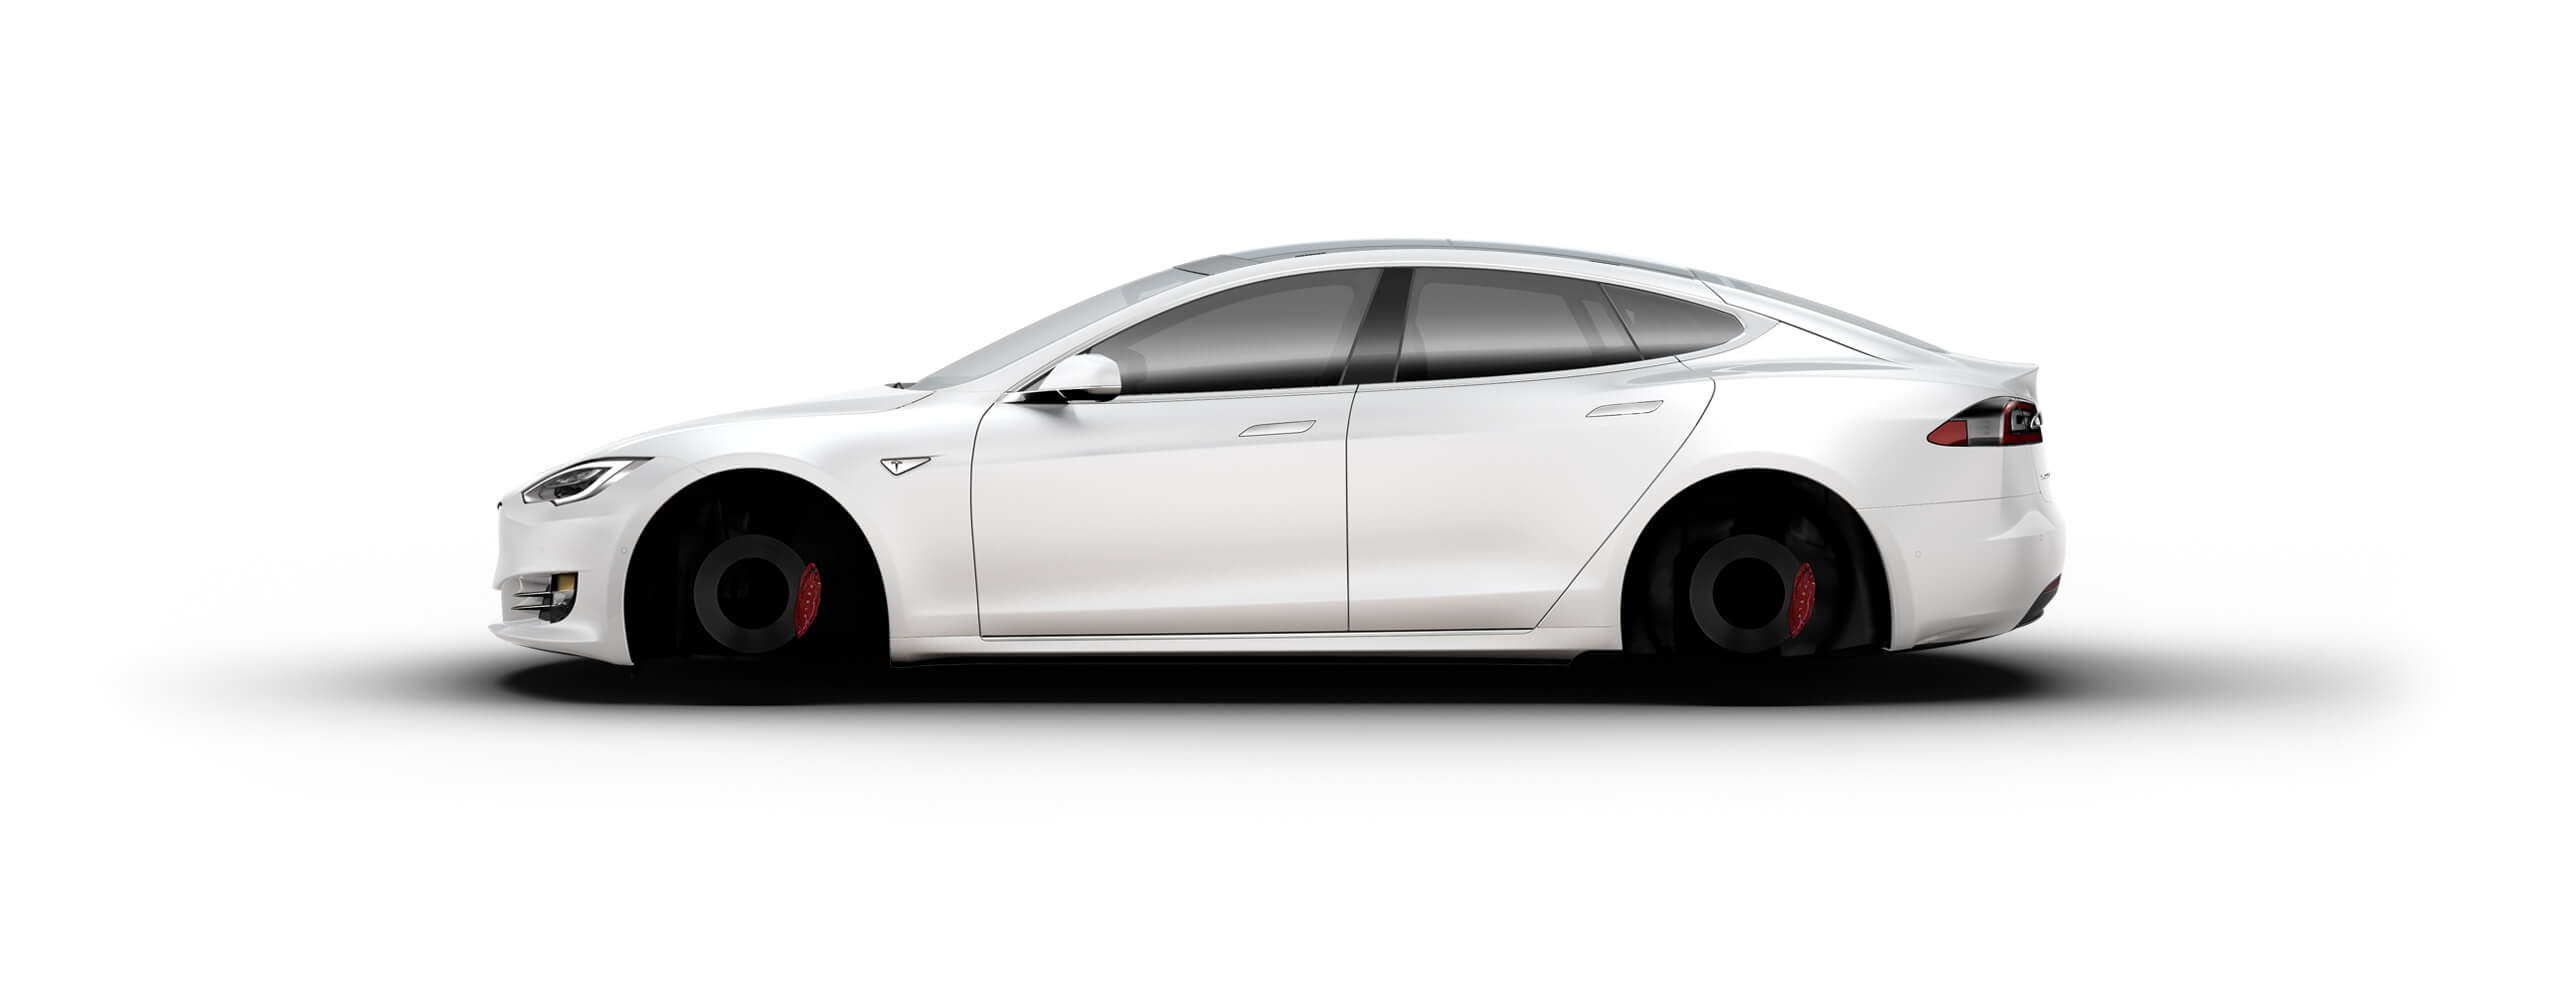
\includegraphics[width=3.5in]{images/car.jpg}
  \end{figure} \pause 
  \begin{itemize}
  \item   作为司机,你会与车有一些互动,如上车、插钥匙、点火、换挡、制动、加速、转向、下车等。你只需要了解车一些基本功能,就可以操纵它。\\
  \item[] 此时,你所看到的是汽车的“逻辑视角”,这些功能通常称为“接口”。 \\[0.1in] \pause 
  
  \item   作为修车师傅,看待汽车的视角就会截然不同。你不仅需要知道如何开车,还必须知道汽车的一些内部细节,比如说发动机如何工作、变速箱如何变速、温度如何控制等等。
  \item[] 这就是“物理视角”,细节发生在“引擎盖下”。
    
  \end{itemize}
\end{frame}

\begin{frame}\ft{\secname}
  \begin{figure}
  	\centering
  	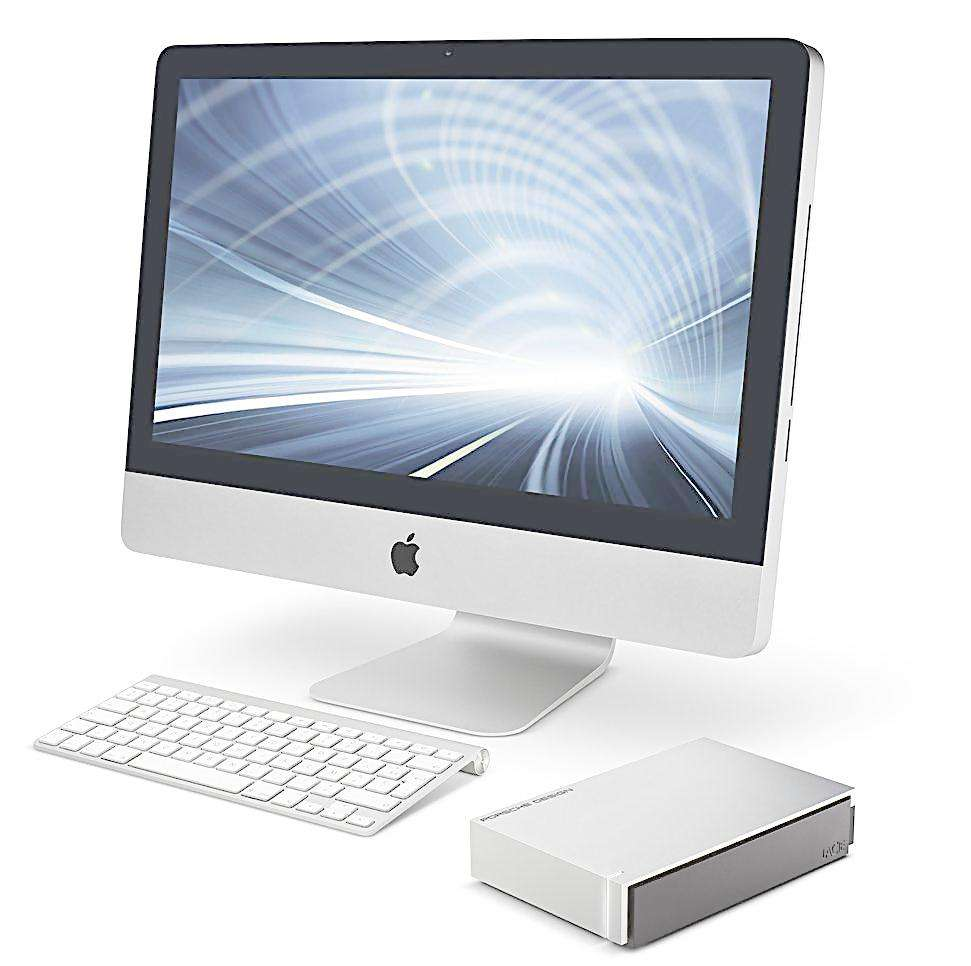
\includegraphics[width=1.5in]{images/computer.jpeg}
  \end{figure} \pause 
  \begin{itemize}
  \item 作为用户,你可以编写文档、收发邮件、上网冲浪、播放音乐、存储图像和玩游戏等,但你并不知道这些APP工作的细节。
  \item[] 此时,你是从逻辑或用户角度看待计算机。 \\[0.1in] \pause 
  \item 作为计算机科学家、程序员、技术支持人员和系统管理员,你看待计算机的角度会截然不同。你必须知道操作系统如何工作、如何配置网络协议、如何编写控制功能的各种脚本。
  \item[] 总之,你必须能够控制底层的细节。

  \end{itemize}

\end{frame}

\begin{frame}[fragile]\ft{\secname}

  作为用户,你不需要知道细节,只需了解接口的工作方式。接口是用户与底层沟通的窗口。

\end{frame}

\begin{frame}[fragile]\ft{\secname}

  看一个抽象的例子---Python 数学模块。一旦导入模块,就可以执行计算
\begin{lstlisting}
  >>> import math
  >>> math.sqrt(16)
  4.0
\end{lstlisting} \pause 

你无需知道计算平方根的细节,只需知道sqrt函数的功能及其使用方式。这就像一个“黑盒子”,其接口可描述为:函数名、参数、返回值,其细节隐藏在内部。
\begin{figure}[htbp]
  \centering
  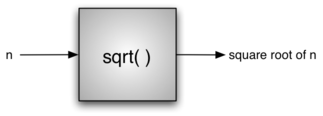
\includegraphics[width=2in]{images/blackbox.png}
\end{figure}

\end{frame}


\section{什么是编程}

\begin{frame}\ft{\secname}
  编程是将算法转换为程序语言的过程,以便能被计算机所执行。

  \begin{itemize}
  \item 首先要有解决方案,亦即算法;
  \item 然后在选择合适的编程语言实现算法。
  \end{itemize}
  计算机科学不研究编程,但编程却是计算机科学家的重要能力。编程通常是解决方案的表达方式。
\end{frame}

\begin{frame}\ft{\secname}
  \begin{itemize}
  \item 算法描述了依据实际问题所生成的解决方案和产生预期结果所需要的一套步骤。

  \item 编程语言必须提供一种表示方法来表示对应的过程和数据。为此,它提供了\red{控制结构}和\red{数据类型}。
  \end{itemize}
\end{frame}

\begin{frame}\ft{\secname}
\red{控制结构}允许以方便而明确的方式表示算法步骤。至少,算法需要执行顺序处理、决策选择和控制迭代。只要语言提供这些基本语句,它就可以表达算法。
\end{frame}

\begin{frame}\ft{\secname}
  在计算机中,所有数据项都由一串一串的二进制数表示。为了让这些二进制串有意义,就需要有\red{数据类型}。 
  \begin{itemize}
  \item 数据类型为二进制数据提供解释,以便我们能够根据实际问题来思考数据。
    这些底层的内置数据类型(有时称为原始数据类型)为算法开发提供了基础。 \pause 
  \item[] 
    例如,大多数编程语言提供整数类型。内存中的二进制数据可解释为整数,并且给予一个与整数(如 23, 654 和 -19)相关联的含义。 \pause \\[0.1in]
  \item   此外,数据类型还提供数据项所参与操作的描述。对于整数,提供诸如加法、减法和乘法的操作。%我们期望数值类型的数据可以参与这些算术运算。
  \end{itemize}
% \end{frame}

% \begin{frame}\ft{\secname}
  
\end{frame}

\begin{frame}\ft{\secname}
  然而,通常我们遇到的困难是问题及其解决方案非常复杂。由语言提供的简单的结构和数据类型,虽然可以表示复杂的解决方案,但在实际中却不好用。
  我们需要一些方法控制这种复杂性,以助于形成更好的解决方案。
\end{frame}
\section{为什么要学习数据结构和抽象数据类型}
\begin{frame}\ft{\secname}
  为管理问题的复杂性及解决过程,计算机科学家使用抽象使他们能够专注于 “大局” 而不会迷失在细节中。\vskip.1in

  通过对问题进行建模,我们能够更好和更有效地解决问题。\vskip.1in


  这些模型允许我们以更加一致的方式来描述我们的算法。
\end{frame}

\begin{frame}\ft{\secname}
  \begin{itemize}
  \item \blue{过程抽象}:隐藏特定函数的细节,以允许用户或客户端在高层查看它。\\[0.1in] \pause 
  \item \blue{数据抽象,即抽象数据类型(ADT)}:对数据和允许操作的逻辑描述,不用考虑如何实现它们。
  \item[] 这意味着我们只关心数据表示什么,而不关心它最终将如何构造。通过提供这种级别的抽象,我们围绕数据创建一个封装。通过封装实现细节,我们将它们从用户的视图中隐藏。这称为信息隐藏。
  \end{itemize}

\end{frame}

\begin{frame}\ft{\secname}

\begin{figure}[htbp]
  \centering
  
\includegraphics[width=4in]{images/ds_adt.png}
  \caption{展示了ADT是什么以及如何操作。用户与接口交互,使用抽象数据类型指定的操作。抽象数据类型是用户与之交互的 shell。实现隐藏在更深的底层。用户不关心实现的细节。}
\end{figure}
\end{frame}

\begin{frame}\ft{\secname}
  ADT的实现要求我们使用一些程序构建和原始数据类型的集合来提供数据的物理视图。

  “逻辑”与“物理”两个视角的分离,允许我们将问题定义复杂的数据模型,而不给出关于模型如何实际构建的细节。
  这提供了独立于实现的数据视图。


  由于通常有许多不同的方法来实现抽象数据类型,所以这种实现独立性允许程序员在不改变数据的用户与其交互的方式的情况下切换实现的细节。

  用户可以继续专注于解决问题的过程。
\end{frame}



\end{document}
